\documentclass{beamer}
\usepackage{tikz}
\usepackage{multicol}
\usepackage[style=authoryear,backend=bibtex]{biblatex}
\addbibresource{ref.bib}

\mode<presentation>
{
	\usetheme[progressbar=foot,numbering=fraction,background=light,block=fill]{metropolis}
	\usecolortheme{default}
	\usefonttheme{default}
	\setbeamertemplate{navigation symbols}{}
	\setbeamertemplate{caption}[numbered]
	\setbeamertemplate{frame footer}{Thomas Pappas | ALMA }
}

% Commands for wrapping properly common expressions.
\newcommand{\indeq}[1]{\stackrel{\text{#1}}{=}}
\newcommand{\RightarrowArg}[1]{\stackrel{#1}{\Rightarrow}}
\newcommand{\LeftrightarrowArg}[1]{\stackrel{#1}{\Leftrightarrow}}
\newcommand{\NE}{\mathrm{N.E.}}
\newcommand{\as}{\mathrm{\alpha_s}}
\newcommand{\R}{\mathbb{R}}
\newcommand{\Gm}{\mathcal{G}}
\DeclareMathOperator*{\argmax}{arg\,max}

\title[]{Pricing Games in Heterogeneous Parallel Networks}
\author[Thomas Pappas]{Thomas Pappas}
\institute[ALMA]{
	\begin{columns}
		\column{0.4\textwidth}
		\begin{figure}
			\centering
			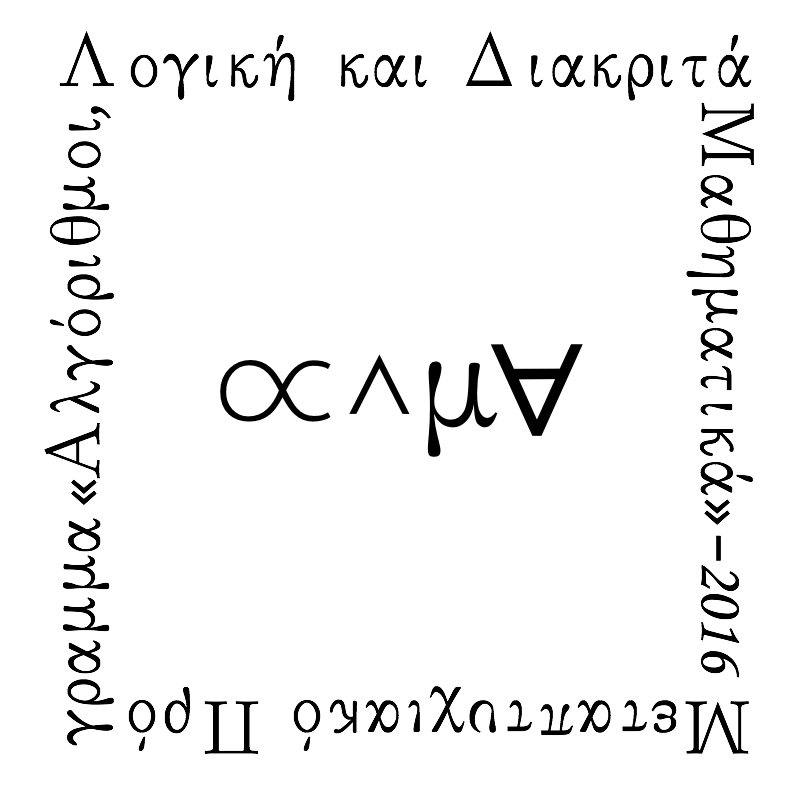
\includegraphics[scale=0.1]{alma.png}
		\end{figure}
		\column{0.5\textwidth}
		ALMA \\
		\tiny{INTER-INSTITUTIONAL GRADUATE PROGRAM \\
			"ALGORITHMS, LOGIC AND DISCRETE MATHEMATICS"}
	\end{columns}
}
\date{\today}

\begin{document}
\AtBeginSection[]{
  \begin{frame}[noframenumbering,plain]
	  \vfill
	  \centering
	  \begin{beamercolorbox}[sep=8pt,center,shadow=true,rounded=true]{title}
	    \usebeamerfont{title}\insertsectionhead\par
	  \end{beamercolorbox}
	  \vfill
  \end{frame}
}


\begin{frame}[noframenumbering,plain]
  \titlepage
\end{frame}

\begin{frame}[noframenumbering,plain]
    \frametitle{Agenda}
    \tableofcontents[hideallsubsections]
\end{frame}


\section{Introduction}

\begin{frame}{History}
	\begin{itemize}
		\item Selfish routing \footcite{pigou1920economics}
		\item Congestion games \footcite{Rosenthal1973ACO}
		\item Wardrop equilibrium \footcite{wardrop_theoretical_1952}
		\item Pricing competition \footcite{10.1287/moor.1060.0231}
		\begin{itemize}
			\item Homogeneous case with toll caps \footcite{Harks_2019}
		\end{itemize}
	\end{itemize}
\end{frame}

\begin{frame}{Our model}
	\begin{center}
		Heterogeneous Non-atomic $n$-link Parallel Network\\
		Toll Congestion Pricing Game
	\end{center}
\end{frame}
\begin{frame}{Our model}
	\begin{center}
		\textbf{Heterogeneous} Non-atomic $n$-link Parallel Network\\
		Toll Congestion \textbf{Pricing} Game
	\end{center}
\end{frame}

\begin{frame}{Our model}
	\;
	\begin{block}{$2$-level optimisation problem}
		\begin{enumerate}
			\item Shelfish routing game, flow on minimum cost paths
			\item Profit maximisation game for link owners
		\end{enumerate}
	\end{block}
\end{frame}

\begin{frame}{Preliminaries}
	\;
	\begin{block}{Non-atomic $n$-link Parallel Network Game}
		A \textbf{Parallel Network} is a directed graph $G = (\{s, t\}, N)$, where $N = \{1, \dots, n\}$ a set of $n$ parallel $s-t$ links.

		For a \textbf{non-atomic} game, a unit of traffic $[0, 1]$, endowed with Lebesque measure $\lambda$, wishes to travel from $s$ to $t$.

		Traffic creates congestion on links and each \textit{player} $p \in [0, 1]$:
		\begin{itemize}
			\item is selfish and wants to experience minimum congestion
			\item has infinitesimal effect on congestion
		\end{itemize}
	\end{block}

	\begin{center}
		\begin{tikzpicture}[scale=0.8, every node/.style={font=\small}]
			% Nodes
			\node[circle, draw, fill=blue!20, minimum size=0.8cm] (s) at (0, 0) {$s$};
			\node[circle, draw, fill=blue!20, minimum size=0.8cm] (t) at (4, 0) {$t$};

			% Edges
			\draw[->, thick] (s) to[bend left=35] node[midway, above] {$1$} (t);
			\draw[->, thick] (s) to[bend left=10] node[midway, above] {$2$} (t);
			\node[align=center] at (2, 0) {$\vdots$};
			\draw[->, thick] (s) to[bend right=35] node[midway, above] {$n$} (t);
		\end{tikzpicture}
	\end{center}
\end{frame}

\begin{frame}{Preliminaries}
	\;
	\begin{block}{Non-atomic $n$-link Parallel Network Game}
		Flow $f: [0, 1] \rightarrow N$ is a Lebesque measurable function assigning players to links.

		\textit{Flow on paths} $x_i = \lambda(\{p \in [0, 1]: f(p) = i\})$
		\begin{itemize}
			\item $x = (x_i)_{i \in N}$ a (stochastic) vector with $x_i \ge 0$ and $\sum_{i \in N} x_i = 1$
		\end{itemize}
		Congestion on links is represented by affine latency functions $(\ell_i)_{i \in N}$ where $\ell_i \in \mathcal{L}_1$, making congestion on link $i$ equal to $\ell_i(x_i)$.
	\end{block}

	\begin{center}
		\begin{tikzpicture}[scale=1.2, every node/.style={font=\small}]
			% Nodes
			\node[circle, draw, fill=blue!20, minimum size=0.8cm] (s) at (0, 0) {$s$};
			\node[circle, draw, fill=blue!20, minimum size=0.8cm] (t) at (4, 0) {$t$};

			% Edges
			\draw[->, thick] (s) to[bend left=35] node[midway, above] {$\ell_1(x_1)$} (t);
			\draw[->, thick] (s) to[bend left=10] node[midway, above] {$\ell_2(x_2)$} (t);
			\node[align=center] at (2, 0) {$\vdots$};
			\draw[->, thick] (s) to[bend right=35] node[midway, above] {$\ell_n(x_n)$} (t);
		\end{tikzpicture}
	\end{center}
\end{frame}

\begin{frame}{Homogeneous players}
	Links can be tolled by assigning tolls $t \in \R_+^N$.

	Player $p$ experiences on link $i$ total cost $c_i(p) = \ell_i(x_i) + t_i$.
	\begin{definition}
		For a given set of tolls $t$, a flow $x$ is a \textit{Wardrop equilibrium for $t$} if $\forall i, j \in N$ with $x_i > 0$ it holds that
		\begin{equation*}
			\ell_i(x_i) + t_i \leq \ell_j(x_j) + t_j
		\end{equation*}
	\end{definition}
	Links with $x_i > 0$ have $\ell_i(x_i) + t_i = K$ for some $K > 0$.

	Wardrop equilibrium always exits and is unique\footcite{??}, denote it by $x(t)$.
\end{frame}

\begin{frame}{Homogeneous players}
	\begin{lemma}[variational inequality\footcite{dafermos1973toll}]
		A flow $x$ is a Wardrop equilibrium for $t$ if and only if for all feasible flows $x^\prime$,
		\[\sum_{i \in N} (\ell_i(x_i) + t_i) \cdot (x_i - x_i^\prime) \leq 0\]
	\end{lemma}
	Equilibrium is indifferent to uniform variations of tolls ($t^\prime = t + c$) or (affine) latencies.
\end{frame}

\begin{frame}{Heterogeneous players}
	Players value time-money differently, so add weight $\alpha$ to money.
	\begin{block}{Distribution function $\alpha: [0, 1] \rightarrow [0, +\infty]$}
		\begin{itemize}
			\item players are ordered w.r.t. sensitivity
			\item $\alpha$ is non-decreasing
		\end{itemize}
	\end{block}
	Player $p$ experiences on link $i$ total cost $c_i(p) = \ell_i(x_i) + \alpha(p) \cdot t_i$.
	\begin{definition}
		For a given set of tolls $t$, a flow $x$ is a \textit{Nash equilibrium for $t$} if for all players $p \in [0, 1]$ and $\forall i \in N$ it holds that
		\begin{equation*}
			c_{f(p)}(p) \leq c_j(p)
		\end{equation*}
	\end{definition}
\end{frame}

\begin{frame}
	Nash equilibrium for $t$ always exists\footcite{1973JSP.....7..295S} and is unique\footcite{MILCHTAICH1996111}, again denote it by $x(t)$.
\end{frame}

\begin{frame}{Pricing competition (2\textsuperscript{nd} level)}
	Links are owned by agents who compete for profit.
	\begin{block}{Profit}
		For given set of tolls $t \in \R_+^N$, link owner $i$ gains profit
		\[\Pi_i(t) = x_i(t) \cdot t_i\]
	\end{block}

	\begin{block}{Best response}
		For fixed tolls assignments from other link owners $t_{-i} = t \setminus \{t_i\}$, link owner $i$ will try and maximise their profit
		\[B_i(t_{-i}) = \argmax_{t_i \ge 0} \Pi(t_i, t_{-i})\]
	\end{block}
\end{frame}

\begin{frame}{Pricing competition (2\textsuperscript{nd} level)}
	\begin{block}{Nash Equilibrium}
		A given set of tolls $t$ is a \textit{Nash Equilibrium for the pricing game} if $\forall i \in N$ and $\forall t_i^\prime \in \R_+$
		\[\Pi_i(t_i, t_{-i}) \geq \Pi_i(t_i^\prime, t_{-i})\]
	\end{block}
	\begin{block}{Nash Equilibrium}
		A given set of tolls $t$ is a \textit{Nash Equilibrium for the pricing game} if
		$\forall i \in N$ we have $|B_i(t_{-i})| = 1$ and
		\[t = (B_i(t_{-i}))_{i \in N}\]
	\end{block}
\end{frame}

\begin{frame}{Game equivalence}
	\begin{definition}[Game equivalence]
		Let $\Gm_1, \Gm_2$ be two $n$-link Network Congestion Games.
		$\Gm_1$ and $\Gm_2$ are called \textbf{equivalent} if and only if for all tolls $t \in \R_+$ it holds that $x^{(1)}(t) = x^{(2)}(t)$, with $x^{(1)}(t), x^{(2)}(t)$ being the Nash Equilibria for $t$ in $\Gm_1, \Gm_2$ respectively.
	\end{definition}
\end{frame}


\section{Heterogeneous players}

\begin{frame}{Heterogeneous players}
	\begin{lemma}
		For $\Gm = (N, \ell, \alpha)$ with tolls $t$ and flow $x(t)$ the Nash equilibrium for $t$, it holds for all $i, j \in N$ with $x_i(t), x_j(t) > 0$ that
		\begin{enumerate}[(i)]
			\item $\ell_i(x_i(t)) < \ell_j(x_j(t))$ iff $t_i > t_j$
			\item $\ell_i(x_i(t)) = \ell_j(x_j(t))$ iff $t_i = t_j$
			\item $\ell_i(x_i(t)) > \ell_j(x_j(t))$ iff $t_i < t_j$
		\end{enumerate}
	\end{lemma}
	\begin{proof}
		Assume $\ell_i(x_i(t)) < \ell_j(x_j(t))$ and $t_i < t_j$ for some $i, j \in N$.
		Then for \textbf{all} players $c_i(p) < c_j(p)$ so $x_j(t) > 0$ is a contradiction.
	\end{proof}
\end{frame}

\begin{frame}{Heterogeneous players}
	Latencies are viewed the same for all players.

	Toll order is the same for all players.

	Tolls define an ordering of the $N$ links where
	\begin{itemize}
		\item $t_1 \ge t_2 \ge \dots \ge t_n$
		\item $\ell_1(x_1(t)) \le \ell_2(x_2(t)) \le \dots \le \ell_n(x_n(t))$
		\item for player representatives from each link $p_1, p_2, \dots, p_n$ we also get $\alpha(p_1) \le \alpha(p_2) \le \dots \le \alpha(p_n)$
	\end{itemize}
	Ordering is unique only when the toll (and therefore also latency) inequalities are strict.
\end{frame}


\section{Sensitivity split}

\begin{frame}{Sensitivity split}
	\begin{definition}
		Let $(N, \ell, \alpha)$ a heterogeneous parallel game, tolls $t$ where $t_i \ne t_j$ for links $i, j \in N$ and $x(t)$ the Nash equilibrium for $t$.
		We define the \textit{money sensitivity split function} $\as^{(i, j)}: \{t \in \R_+^N|t_i \ne t_j\} \rightarrow (0, +\infty)$ as
		\[\as^{(i, j)}(t) = \frac{\ell_j(x_j(t)) - \ell_i(x_i(t))}{t_i - t_j}\]
	\end{definition}
\end{frame}

\begin{frame}{Sensitivity split}
	\begin{block}{Properties}
		περιεχόμενο...
	\end{block}
\end{frame}

\begin{frame}{Sensitivity split}
	\begin{block}{Monotonicity}
		περιεχόμενο...
	\end{block}
\end{frame}

\begin{frame}{Sensitivity split}
	Characterisation.
\end{frame}


\section{Pseudo-heterogeneous Pricing Games}

\section{Step distribution function}

\section{Future work}

\begin{frame}[noframenumbering,plain]{}
	\centering
    \huge Thank you!\\
    \normalsize Thomas Pappas\\
    thpappas@di.uoa.gr
\end{frame}

\end{document}
